\documentclass[tikz]{standalone}

\usepackage{amsmath} % for \text
\usepackage{xfrac} % for \myfrac
\usepackage{bm} % for \bm
\usetikzlibrary{calc}
\usetikzlibrary{positioning}
\usetikzlibrary{decorations.pathreplacing,decorations.markings}
\usetikzlibrary{patterns} % 加载 patterns 库
\usepackage{comment}


\colorlet{myred}{red!80!black}
\colorlet{myblue}{blue!80!black}
\colorlet{mygreen}{green!60!black}
\colorlet{myorange}{orange!70!red!60!black}
\colorlet{mydarkred}{red!30!black}
\colorlet{mydarkblue}{blue!40!black}
\colorlet{mydarkgreen}{green!30!black}
\colorlet{myred2}{red!50!white}

\colorlet{mylightblue}{blue!60!cyan!80!black!15}
\colorlet{mypurple}{blue!50!red!70}
\colorlet{gaugecol}{red!90!black!70} % Wiki red
\colorlet{leptoncol}{green!80!black!70} % Wiki green
\colorlet{quarkcol}{blue!85!cyan!95!black!55} % Wiki purple
\colorlet{quarkred}{red!98!black!55} % quark red
\colorlet{quarkblue}{blue!85!cyan!98!black!55} % quark blue
\colorlet{quarkgreen}{green!95!black!55} % quark green
\colorlet{gluoncyan}{cyan!100!black!55} % gluon cyan
\colorlet{gluongreen}{green!75!blue!95!black!70} % gluon green
\colorlet{gluonyellow}{yellow!98!black!55} % gluon yellow
\colorlet{gluonorange}{orange!100!black!65} % gluon orange
\colorlet{gluonmagenta}{magenta!100!black!70} % gluon magenta
\colorlet{scalarcol}{yellow!70!orange!98!black}
\colorlet{tensorcol}{blue!50!red!70} % Wiki light blue
\colorlet{groupcol}{orange!15}

\tikzset{
    mynode/.style={
        circle,        % 形状为圆形
        fill=black,    % 填充颜色为黑色
        inner sep=0.4, % 点的大小
        draw           % 添加边框
    }
}


\begin{document}

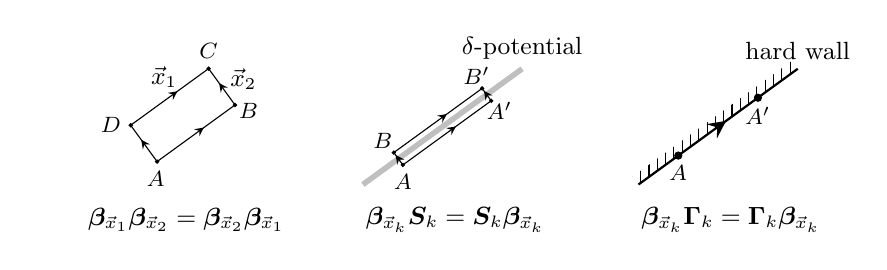
\begin{tikzpicture}[x=2.5cm, y=2.5cm]

\def\th{36}
\def\rr{0.27}
\def\rrr{0.28}
\def\phi{25}
\def\phit{8}
\def\thth{36}
\def\shift{1.4}
\def\shiftshift{2.8}
\def\De{0.05}
\def\Dy{-0.18}
% 定义点
\coordinate (P1) at (0, 0);

\pgfmathsetmacro{\x}{cos(\th)}
\pgfmathsetmacro{\y}{sin(\th)}
\coordinate (P2) at (1.0*\x, 1.0*\y);

\pgfmathsetmacro{\x}{cos(\th)/2*1.2 + \rr*cos(\th+\phi)}
\pgfmathsetmacro{\y}{sin(\th)/2*1.2 + \rr*sin(\th+\phi)}
\coordinate (Q1) at (\x, \y);

\pgfmathsetmacro{\x}{cos(\th)/2*1.2 + \rr*cos(180+\th-\phi)}
\pgfmathsetmacro{\y}{sin(\th)/2*1.2 + \rr*sin(180+\th-\phi)}
\coordinate (Q2) at (\x, \y);

\pgfmathsetmacro{\x}{cos(\th)/2*1.2 + 0.5*(\rr*cos(\th+\phi)+\rr*cos(180+\th-\phi))}
\pgfmathsetmacro{\y}{sin(\th)/2*1.2 + 0.5*(\rr*sin(\th+\phi)+\rr*sin(180+\th-\phi))}
\coordinate (Q12) at (\x, \y);

\pgfmathsetmacro{\x}{cos(\th)/2*1.2 + \rr*cos(180+\th+\phi)}
\pgfmathsetmacro{\y}{sin(\th)/2*1.2 + \rr*sin(180+\th+\phi)}
\coordinate (Q3) at (\x, \y);

\pgfmathsetmacro{\x}{cos(\th)/2*1.2 + \rr*cos(\th-\phi)}
\pgfmathsetmacro{\y}{sin(\th)/2*1.2 + \rr*sin(\th-\phi)}
\coordinate (Q4) at (\x, \y);

\node[mynode] at (Q1) {};
\node[mynode] at (Q2) {};
\node[mynode] at (Q3) {};
\node[mynode] at (Q4) {};
%\draw[postaction={decorate}] (P1) -- (P2);
\draw[postaction={decorate}, 
      decoration={markings, mark=at position 0.6 with {\arrow{stealth}}}] (Q2) -- (Q1);
\draw[postaction={decorate}, 
      decoration={markings, mark=at position 0.6 with {\arrow{stealth}}}] (Q3) -- (Q2);
\draw[postaction={decorate}, 
      decoration={markings, mark=at position 0.6 with {\arrow{stealth}}}] (Q3) -- (Q4);
\draw[postaction={decorate}, 
      decoration={markings, mark=at position 0.6 with {\arrow{stealth}}}] (Q4) -- (Q1);

\node[above, xshift=0pt] at (Q1) {\footnotesize $C$};
\node[left, xshift=0pt] at (Q2) {\footnotesize $D$};
\node[below, xshift=-0.5] at (Q3) {\footnotesize $A$};
\node[right, xshift=-2, yshift=-2] at (Q4) {\footnotesize $B$};

\node[above, xshift=-2, yshift=-0] at (Q12) {\small $\vec{x}_1$};
\node[above, xshift=3, yshift=2] at (Q4) {\small $\vec{x}_2$};

\pgfmathsetmacro{\x}{0.5*(0.1 + 0.8*cos(\th))}
\pgfmathsetmacro{\y}{\Dy}
\coordinate (P01) at (\x,\y);

\pgfmathsetmacro{\x}{\shift}
\pgfmathsetmacro{\y}{0}
\coordinate (P3) at (\x, \y);

\pgfmathsetmacro{\x}{cos(\thth)+\shift}
\pgfmathsetmacro{\y}{sin(\thth)}
\coordinate (P4) at (\x, \y);

\pgfmathsetmacro{\x}{\shift + cos(\th)/2*1 + \rrr*cos(\th+\phit)}
\pgfmathsetmacro{\y}{sin(\th)/2*1 + \rrr*sin(\th+\phit)}
\coordinate (Q5) at (\x, \y);

\pgfmathsetmacro{\x}{\shift + cos(\th)/2*1 + \rrr*cos(180+\th-\phit)}
\pgfmathsetmacro{\y}{sin(\th)/2*1 + \rrr*sin(180+\th-\phit)}
\coordinate (Q6) at (\x, \y);

\pgfmathsetmacro{\x}{\shift + cos(\th)/2*1 + 0.5*(\rrr*cos(\th+\phit)+\rrr*cos(180+\th-\phit))}
\pgfmathsetmacro{\y}{sin(\th)/2*1 + 0.5*(\rrr*sin(\th+\phit)+\rrr*sin(180+\th-\phit))}
\coordinate (Q56) at (\x, \y);

\pgfmathsetmacro{\x}{\shift + cos(\th)/2*1 + \rrr*cos(180+\th+\phit)}
\pgfmathsetmacro{\y}{sin(\th)/2*1 + \rrr*sin(180+\th+\phit)}
\coordinate (Q7) at (\x, \y);

\pgfmathsetmacro{\x}{\shift + cos(\th)/2*1 + \rrr*cos(\th-\phit)}
\pgfmathsetmacro{\y}{sin(\th)/2*1 + \rrr*sin(\th-\phit)}
\coordinate (Q8) at (\x, \y);


\pgfmathsetmacro{\x}{cos(\thth)+\shift+0.1}
\pgfmathsetmacro{\y}{sin(\thth)*0.2}
\coordinate (PS0) at (\x, \y);

\pgfmathsetmacro{\x}{cos(\thth)+\shift+0.1 + 0.2*cos(\thth + 90)}
\pgfmathsetmacro{\y}{sin(\thth)*0.2 + 0.2*sin(\thth + 90)}
\coordinate (PS2) at (\x, \y);

\pgfmathsetmacro{\x}{cos(\thth)+\shift+0.1 + 0.2*cos(\thth)}
\pgfmathsetmacro{\y}{sin(\thth)*0.2 + 0.2*sin(\thth)}
\coordinate (PS1) at (\x, \y);

\pgfmathsetmacro{\x}{cos(\thth)/2-\De*cos(\thth+90)+\shift}
\pgfmathsetmacro{\y}{sin(\thth)/2-\De*sin(\thth+90)}
\coordinate (P5) at (\x, \y);

\pgfmathsetmacro{\x}{cos(\thth)/2+\De*cos(\thth+90)+\shift}
\pgfmathsetmacro{\y}{sin(\thth)/2+\De*sin(\thth+90)}
\coordinate (P6) at (\x, \y);

\pgfmathsetmacro{\x}{0.5*(0.0 + 1.0*cos(\thth)) + \shift}
\pgfmathsetmacro{\y}{\Dy}
\coordinate (P02) at (\x,\y);

\pgfmathsetmacro{\x}{\shiftshift}
\pgfmathsetmacro{\y}{0}
\coordinate (P7) at (\x, \y);

\pgfmathsetmacro{\x}{cos(\thth)+\shiftshift}
\pgfmathsetmacro{\y}{sin(\thth)}
\coordinate (P8) at (\x, \y);

\pgfmathsetmacro{\x}{cos(\thth)+\De*cos(\thth+90)+\shiftshift}
\pgfmathsetmacro{\y}{sin(\thth)+\De*sin(\thth+90)}
\coordinate (P9) at (\x, \y);

\pgfmathsetmacro{\x}{\De*cos(\thth+90)+\shiftshift}
\pgfmathsetmacro{\y}{\De*sin(\thth+90)}
\coordinate (P10) at (\x, \y);

\pgfmathsetmacro{\x}{cos(\thth)/2+\shiftshift}
\pgfmathsetmacro{\y}{sin(\thth)/2}
\coordinate (P11) at (\x, \y);

\pgfmathsetmacro{\x}{cos(\thth)*0.25+\shiftshift}
\pgfmathsetmacro{\y}{sin(\thth)*0.25}
\coordinate (Q9) at (\x, \y);

\pgfmathsetmacro{\x}{cos(\thth)*0.75+\shiftshift}
\pgfmathsetmacro{\y}{sin(\thth)*0.75}
\coordinate (Q10) at (\x, \y);

\pgfmathsetmacro{\x}{0.5*(0.0 + 1.0*cos(\thth)) + \shiftshift}
\pgfmathsetmacro{\y}{\Dy}
\coordinate (P03) at (\x,\y);

%\node[mynode] at (P1) {};
%\node[mynode] at (P2) {};
%\node[above] at (P2) {\small propagating};



\draw[gray!50, line width=2.0] (P3) -- (P4);
\node[mynode] at (Q5) {};
\node[mynode] at (Q6) {};
\node[mynode] at (Q7) {};
\node[mynode] at (Q8) {};
\node[above] at (P4) {\small $\delta$-potential};
\node[above, yshift=-2, xshift = -2] at (Q5) {\footnotesize $B^\prime$};
\node[above, yshift=-2, xshift=-4] at (Q6) {\footnotesize $B$};
\node[below] at (Q7) {\footnotesize $A$};
\node[below, xshift = 3, yshift = 3] at (Q8) {\footnotesize $A^\prime$};
\draw[postaction={decorate}, 
      decoration={markings, mark=at position 0.6 with {\arrow{stealth}}}] (Q6) -- (Q5);
\draw[postaction={decorate}, 
      decoration={markings, mark=at position 0.6 with {\arrow{stealth}}}] (Q7) -- (Q8);
\draw[postaction={decorate}, 
      decoration={markings, mark=at position 0.8 with {\arrow{stealth}}}] (Q7) -- (Q6);
\draw[postaction={decorate}, 
      decoration={markings, mark=at position 0.8 with {\arrow{stealth}}}] (Q8) -- (Q5);

\fill[pattern=vertical lines, pattern color=black] (P7) -- (P8) -- (P9) -- (P10) -- cycle;
\draw[black, thick] (P7) -- (P8);

\node[circle,        % 形状为圆形
        fill=black,    % 填充颜色为黑色
        inner sep=0.9, % 点的大小
        draw   ] at (Q9) {};
\node[below] at (Q9) {\footnotesize $A$};

\node[circle,        % 形状为圆形
        fill=black,    % 填充颜色为黑色
        inner sep=0.9, % 点的大小
        draw   ] at (Q10) {};
\node[below] at (Q10) {\footnotesize $A^\prime$};

\draw[postaction={decorate}, 
      decoration={markings, mark=at position 0.6 with {\arrow[scale=2]{stealth}}}] (Q9) -- (Q10);


\node[above] at (P8) {\small hard wall};

\node[] at (P01) {\small $\quad \quad \bm{\beta}_{\vec{x}_1}\bm{\beta}_{\vec{x}_2}=\bm{\beta}_{\vec{x}_2}\bm{\beta}_{\vec{x}_1}$};
\node[] at (P02) {\small \quad $\bm{\beta}_{\vec{x}_k} \bm{S}_{k}
= \bm{S}_{k} \bm{\beta}_{\vec{x}_k}$};
\node[] at (P03) {\small \quad $\bm{\beta}_{\vec{x}_k}\bm{\Gamma}_k
= \bm{\Gamma}_k \bm{\beta}_{\vec{x}_k} $};

% \node[] at (PS0) {\tiny k};


      


 
\end{tikzpicture}




\end{document}